The detection of foodborne hazards has seen great advancements with the introduction of sensors and biosensors \citep{guRecent2022,liResearch2022}. Sensors are defined by the International Union of Pure and Applied Chemistry (IUPAC) as devices that transform chemical information into detectable signals \citep{hulanickiChemical1991} and are becoming more widespread across all sectors of analytical science; they are particularly relevant in those fields where rapid, accurate detection is crucial, as in the case of food safety, where illnesses can be prevented in favour of public health \citep{payneSensors1983, javaidSensors2021, baranwalElectrochemical2022}.

\paragraph{Components and mechanisms of sensors}
\begin{figure}[ht]
	\centering
	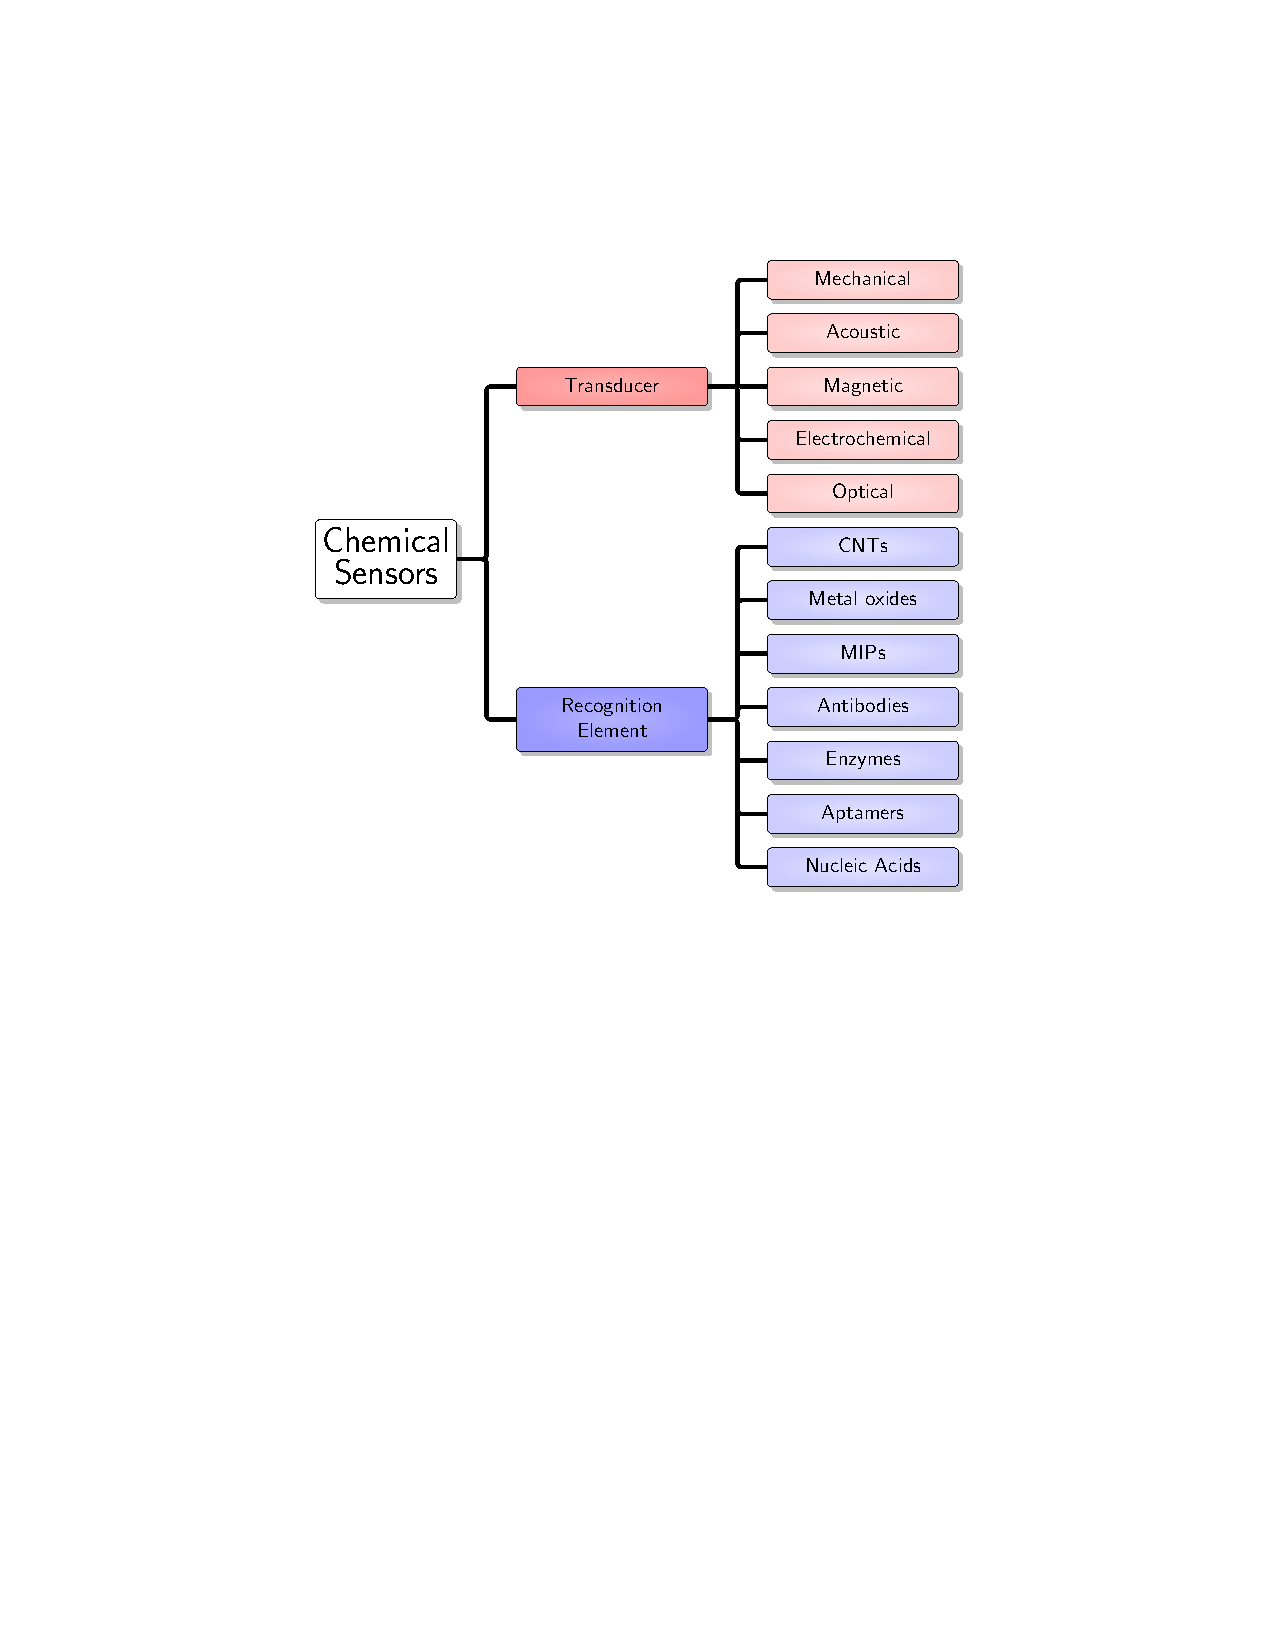
\includegraphics[width=0.5\textwidth]{figures/chapter1/sensors/Fig2_SensorClass.pdf}
	\caption{Classification of chemical sensors based on their recognition elements and transduction method. The recognition element selectively interacts with the target analyte and can be composed of biological (nucleic acids, aptamers, enzymes, antibodies) or synthetic materials (molecularly imprinted polymers (MIPs), metal oxides, carbon nanotubes (CNTs)). The transducer converts the interaction with the analyte into a measurable signal that can be optical, electrochemical, magnetic, acoustic, or mechanical. This figure is reproduced from \note{insert my histamine paper identifier}}.
	\label{fig:sensorClass}
\end{figure}

Sensors typically consist of two components: a recognition element and a signal transducer. The recognition element interacts specifically with the analyte of interest, while the signal transducer converts this interaction into a measurable signal; this signal can take many forms, for example electrical currents, optical or acoustic changes, thus allowing to accomodate for a wide range of detection mechanisms \citep{hulanickiChemical1991,mehrotraBiosensors2016}. Biosensors refer to a subgroup of sensors that use biological recognition elements to detect the target analytes \citep{nagelGlossary1992}; they are particularly suited for detecting biological elements, such as whole cells, viruses, and simpler biomolecules (nucleic acids, proteins, vitamines and hormones), thanks to their high specificity and sensitivity \citep{mehrotraBiosensors2016}.

Recognition elements can be categorized as physical, chemical, and biochemical. Physical recognition elements detect measurable changes in properties such as absorbance, mass, or temperature upon interacting with an analyte. Chemical recognition elements induce reactions that generate detectable products, like electrons. Biochemical recognition elements have a biological origin, like enzymes, antibodies, and nucleic acids, and are mainly used for biological target analytes.

Sensors can be further categorized based on their transduction methods. These include electrochemical transduction, which deals with changes in current or potential; optical transduction, which is based on variations in light properties like fluorescence or absorbance; acoustic transduction, which tracks shifts in sound waves; and lastly mechanical transduction, which responds to changes in physical properties, for example tracking the movement of the target analyte. A summary of the components of (bio)sensors is visible in Figure \ref{fig:sensorClass}.

\subparagraph{Transducers}
Signal transduction can take various forms depending on the objective of the sensor, the analyte of interest, and the recognition element used. The two most commonly employed strategies are optical and electrochemical transduction.

Optical transduction relies on phenomena such as absorbance, reflectance, luminescence, fluorescence, refractive index changes, or light scattering to generate detectable signals \citep{danchukOptical2020}. This approach is particularly advantageous when small sample volumes are required, and it enables rapid, reproducible, and even multiplexed detection \citep{chenOptical2020}. However, these techniques can face limitations in terms of portability; indeed instruments such as spectrometers and spectrofluorometers are bulky, confining them to laboratory use and limiting their on-site application \citep{elsherifOptical2022}. Other drawbacks of optical sensors include limited sensitivity and recognition elements available \citep{yanReview2018}, high costs, low processing speeds for large datasets \citep{al-ashwalDeep2023}, and the potential alteration of sample composition in certain applications \citep{ignestiNew2016}.

Electrochemical transduction is based on the generation of an electric signal, which can generally occur either as a faradaic or non-faradaic response. A faradaic response involves electron transfer processes that generate a measurable current or impedance change, often influenced by redox reactions catalyzed by the recognition element upon interaction with the analyte \citep{adamExploring2024}. A non-faradaic response involves surface interactions between the electrodes and the desired analyte causing changes in capacitance and impedance without redox reactions; this allows for label-free, sensitive, and reproducible detection of analytes \citep{kellNonFaradaic1991}. Among the strategies adopted for the detection of foodborne hazards using electrochemical sensors, voltammetric measurements, which monitor current as a function of a variable potential, and amperometric measurements, where current is measured under a fixed potential bias, are the most prevalent. Less commonly employed, though still notable, are potentiometric measurements, which evaluate changes in electric potential in the absence of current flow \citep{hulanickiChemical1991}.

Amid debates about nomenclature and classification, field-effect transistors (FETs), and more specifically, electrolyte-gated field-effect transistors (EG-FETs) are gaining traction in the development of new (bio)sensors \citep{minamikiExtendedgate2015, nakatsukaAptamer2018, shkodraElectrolytegated2021}, described in detail in Section \ref{sec:FET}. In brief, these are three-electrode platforms that significantly amplify the signal while maintaining low operating voltages. This makes them particularly attractive for detecting biological molecules for a few reasons: these analytes are typically present in low concentrations in samples and a high amplification is needed to accurately detect them; moreover, the analyte can remain in an environment closely resembling its natural state (aqueous environment) and is not damaged by high voltages or currents. Other advantages include their robustness and miniaturization possibilities, making them suitable for field measurements with good sensitivity and selectivity \citep{grieshaberElectrochemical2008}; nevertheless, they remain susceptible to cross-reactivity in complex matrices and their shelf life is still limited due to sensitivity to environmental factors such as temperature and humidity and potential surface adsorption of impurities \citep{fleetElectrochemical1992, williamsElectrochemical2020}.

\subparagraph{Recognition elements}
Recognition elements play a central role in sensors, conferring selectivity for the analyte of interest and enhancing sensitivity. Since the library of recognition elements is remarkably extensive and often analyte-specific, a comprehensive list cannot be compiled; this section aims to provide an overview of the most commonly used types, as shown in Figure \ref{fig:recognitionElements}.

First of all, recognition elements can be divided into two categories based on their origin: chemical recognition elements, which are generally based on inorganic or organic chemical synthesis, and biological recognition elements, which are molecules of biological origin, mostly used for the detection of biomolecules.

Among chemical recognition elements, metal oxides are noteworthy thanks to their enzyme-like functions, \eg{} oxidase-like activities \citep{poolakkandyTransition2021}. These molecules catalyze the oxidation of the substrate, which donates electrons to oxygen, thus forming \ce{H2O} or \ce{H2O2}; \ce{H2O2} is then reduced at the electrode surface under a constant potential generating a detectable signal that depends on the analyte itself \citep{liuReview2021}.

Another widely used class of chemical recognition elements is that of molecularly imprinted polymers (MIPs): these are synthetic recognition elements known for their cost-effectiveness, high stability, and resilience under harsh conditions \citep{uzunMolecularlyimprinted2016}. Indeed, these polymers are molded using the target analyte as template molecule to create cavities tailored to its size, shape, and interaction points; this allows high selectivity and reliability in sensing applications \citep{hassanBiomimetic2019}.

Building on the idea of specificity, affinity-based recognition relies on the specific interactions between a recognition element and the target analyte, with mechanisms that are often driven by electrostatic interactions or hydrogen bonding. An example of such recognition is the use of nickel ions (\ce{Ni^{2+}}), which exhibit a specific affinity for the imidazole ring found in biological molecules, such as histamine \citep{fukushimaColorimetric2021}.

At the forefront of biological recognition elements there are antibodies: these are widely employed thanks to their exceptional specificity and sensitivity \citep{shkodraElectrolytegated2021}. Structurally, they consist of two heavy and two light chains linked by disulfide bonds in a Y shape, with the paratope located at the terminal ends of the arms responsible for recognizing specific epitopes on the target analyte \citep{moralesGuide2018}. While versatile and effective, antibodies are bulky molecules: this can make the detection challenging when working with sensors governed by the Debye length \citep{nakatsukaAptamer2018, shkodraElectrolytegated2021}. To overcome this limitation, antibody fragments, such as Fab fragments, can be cleaved using pepsin protease; the smaller fragments retain the paratope fraction of the receptor, thus maintaining the ability to bind the target while reducing steric hindrance \citep{crivianu-gaitaAptamers2016}.
%
Another promising biological recognition element is represented by aptamers: these are short nucleotide sequences carefully assembled to bind target analytes with high specificity and affinity \citep{shkodraElectrolytegated2021}. Upon interaction with the analyte, aptamers undergo conformational changes which modify the distribution of negative charges along the backbone, thus generating a detectable signal \citep{nakatsukaAptamer2018}. Despite their high chemical stability, aptamers may not be the appropriate choice for a sensor due to their complex and costly synthesis: indeed, after nucleotide assembly, the filaments must undergo a labor-intensive process for optimizing aptamer-target interactions, that is Systematic Evolution of Ligands by Exponential Enrichment (SELEX) \citep{ellingtonVitro1990, tuerkSystematic1990}.
%
Finally, enzymes are a subgroup of proteins that can selectively bind their analytes through electrostatic forces, hydrogen bonding, and other non-covalent interactions, and catalyze a reaction (cfr. metal oxides). The characteristic that makes them attractive as biorecognition elements for sensors is their ability to regenerate in physiological conditions, thus paving the way for the development of reusable sensors \citep{bocanegra-rodriguezNew2020}. Despite this, their main limitation lies in their low stability, as they are prone to denaturation when exposed to changes in pH or temperature \citep{herletNew2017}.

\begin{figure}[!ht]
    \centering
    %\hfill
    \subfloat[Nanozymes]{%
        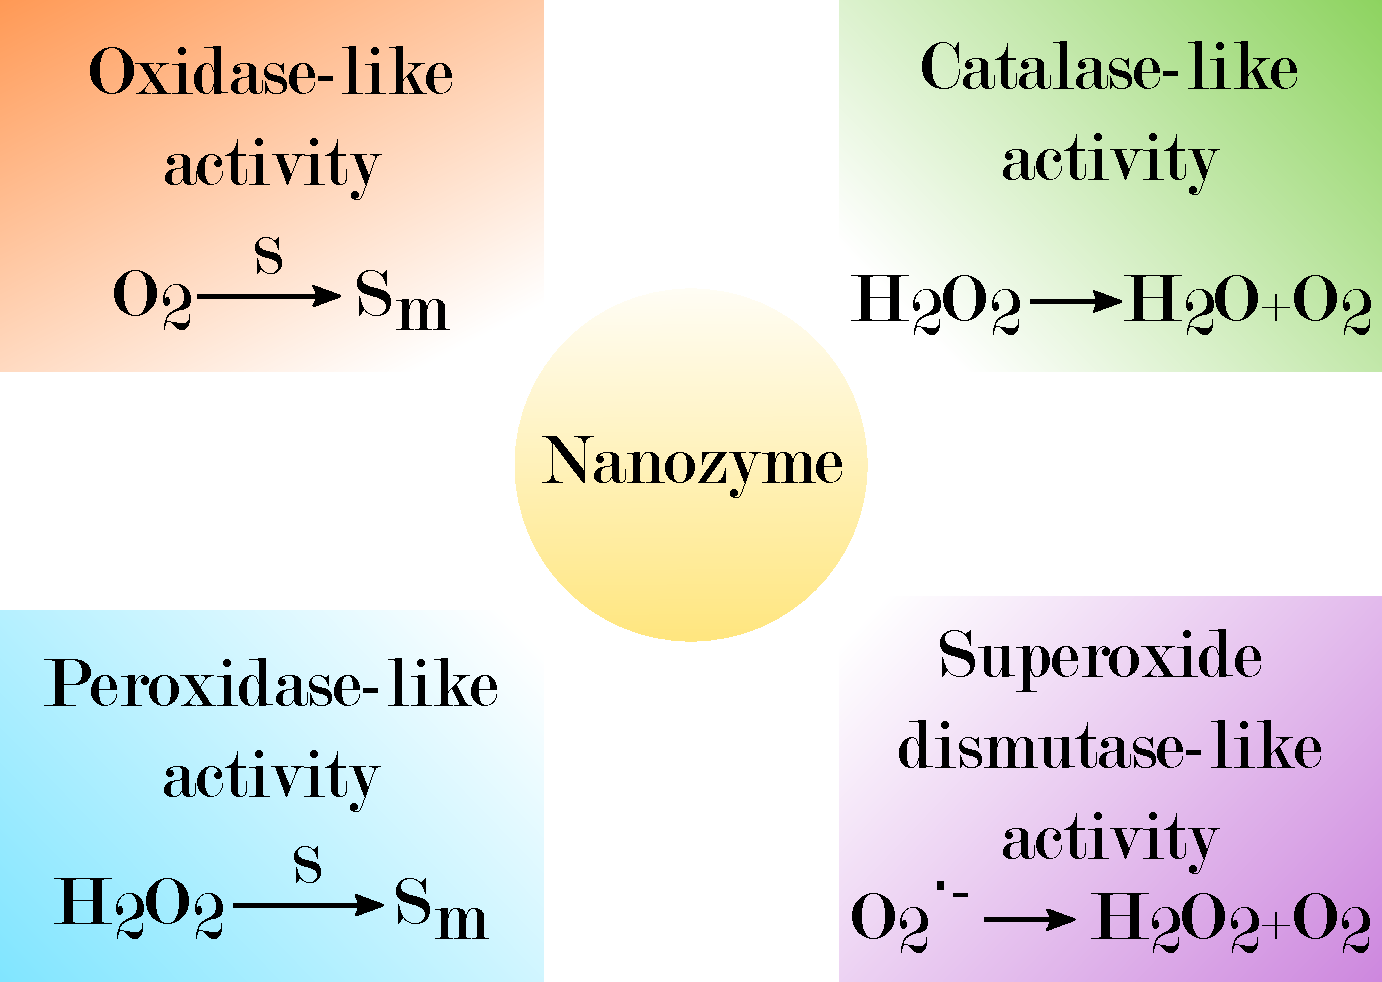
\includegraphics[width=0.3\textwidth]{figures/chapter1/sensors/Fig1_Nanozymes.pdf}
        \label{fig:nano}
    }
    %
    \hspace{0.05\textwidth}
    %
    \subfloat[Molecularly Imprinted Polymers]{%
    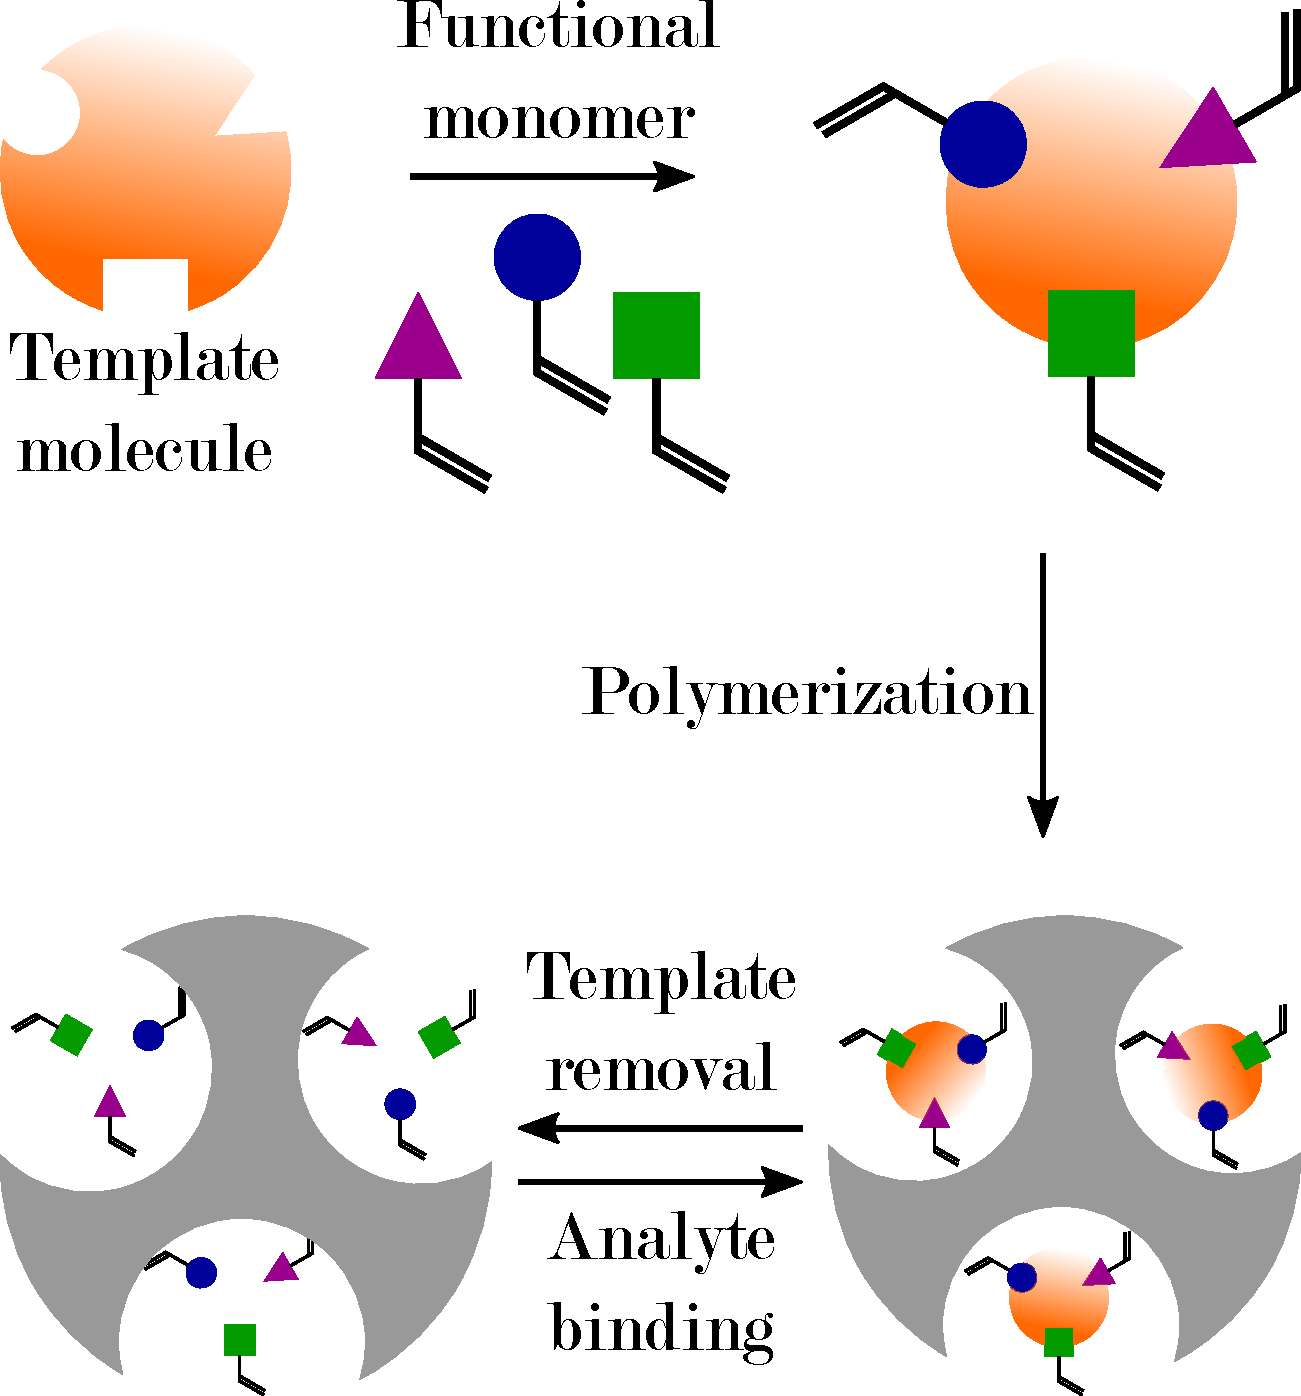
\includegraphics[width=0.3\textwidth]{figures/chapter1/sensors/Fig1_MIPs.pdf}
    \label{fig:mips}
    }
    %
    \vskip 1em
    %
    \subfloat[Antibodies]{%
        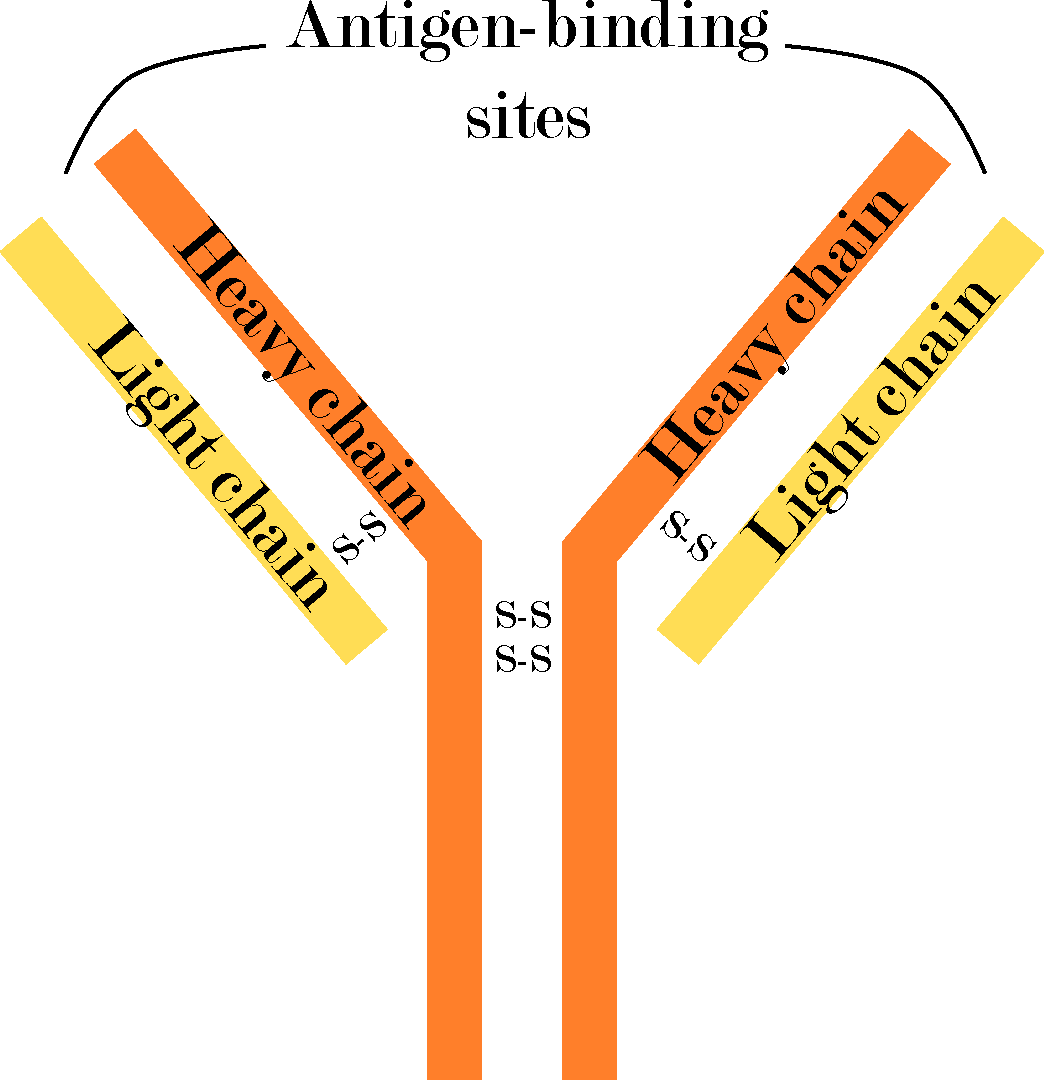
\includegraphics[width=0.3\textwidth]{figures/chapter1/sensors/Fig1_Antibody.pdf}
        \label{fig:ab}
    }
    \hfill
    \subfloat[Enzymes]{%
        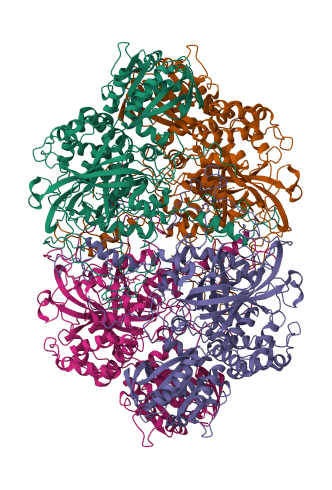
\includegraphics[width=0.3\textwidth]{figures/chapter1/sensors/Fig1_Enzyme.png}
        \label{fig:enz}
    }
    \hfill
    \subfloat[Aptamers]{%
        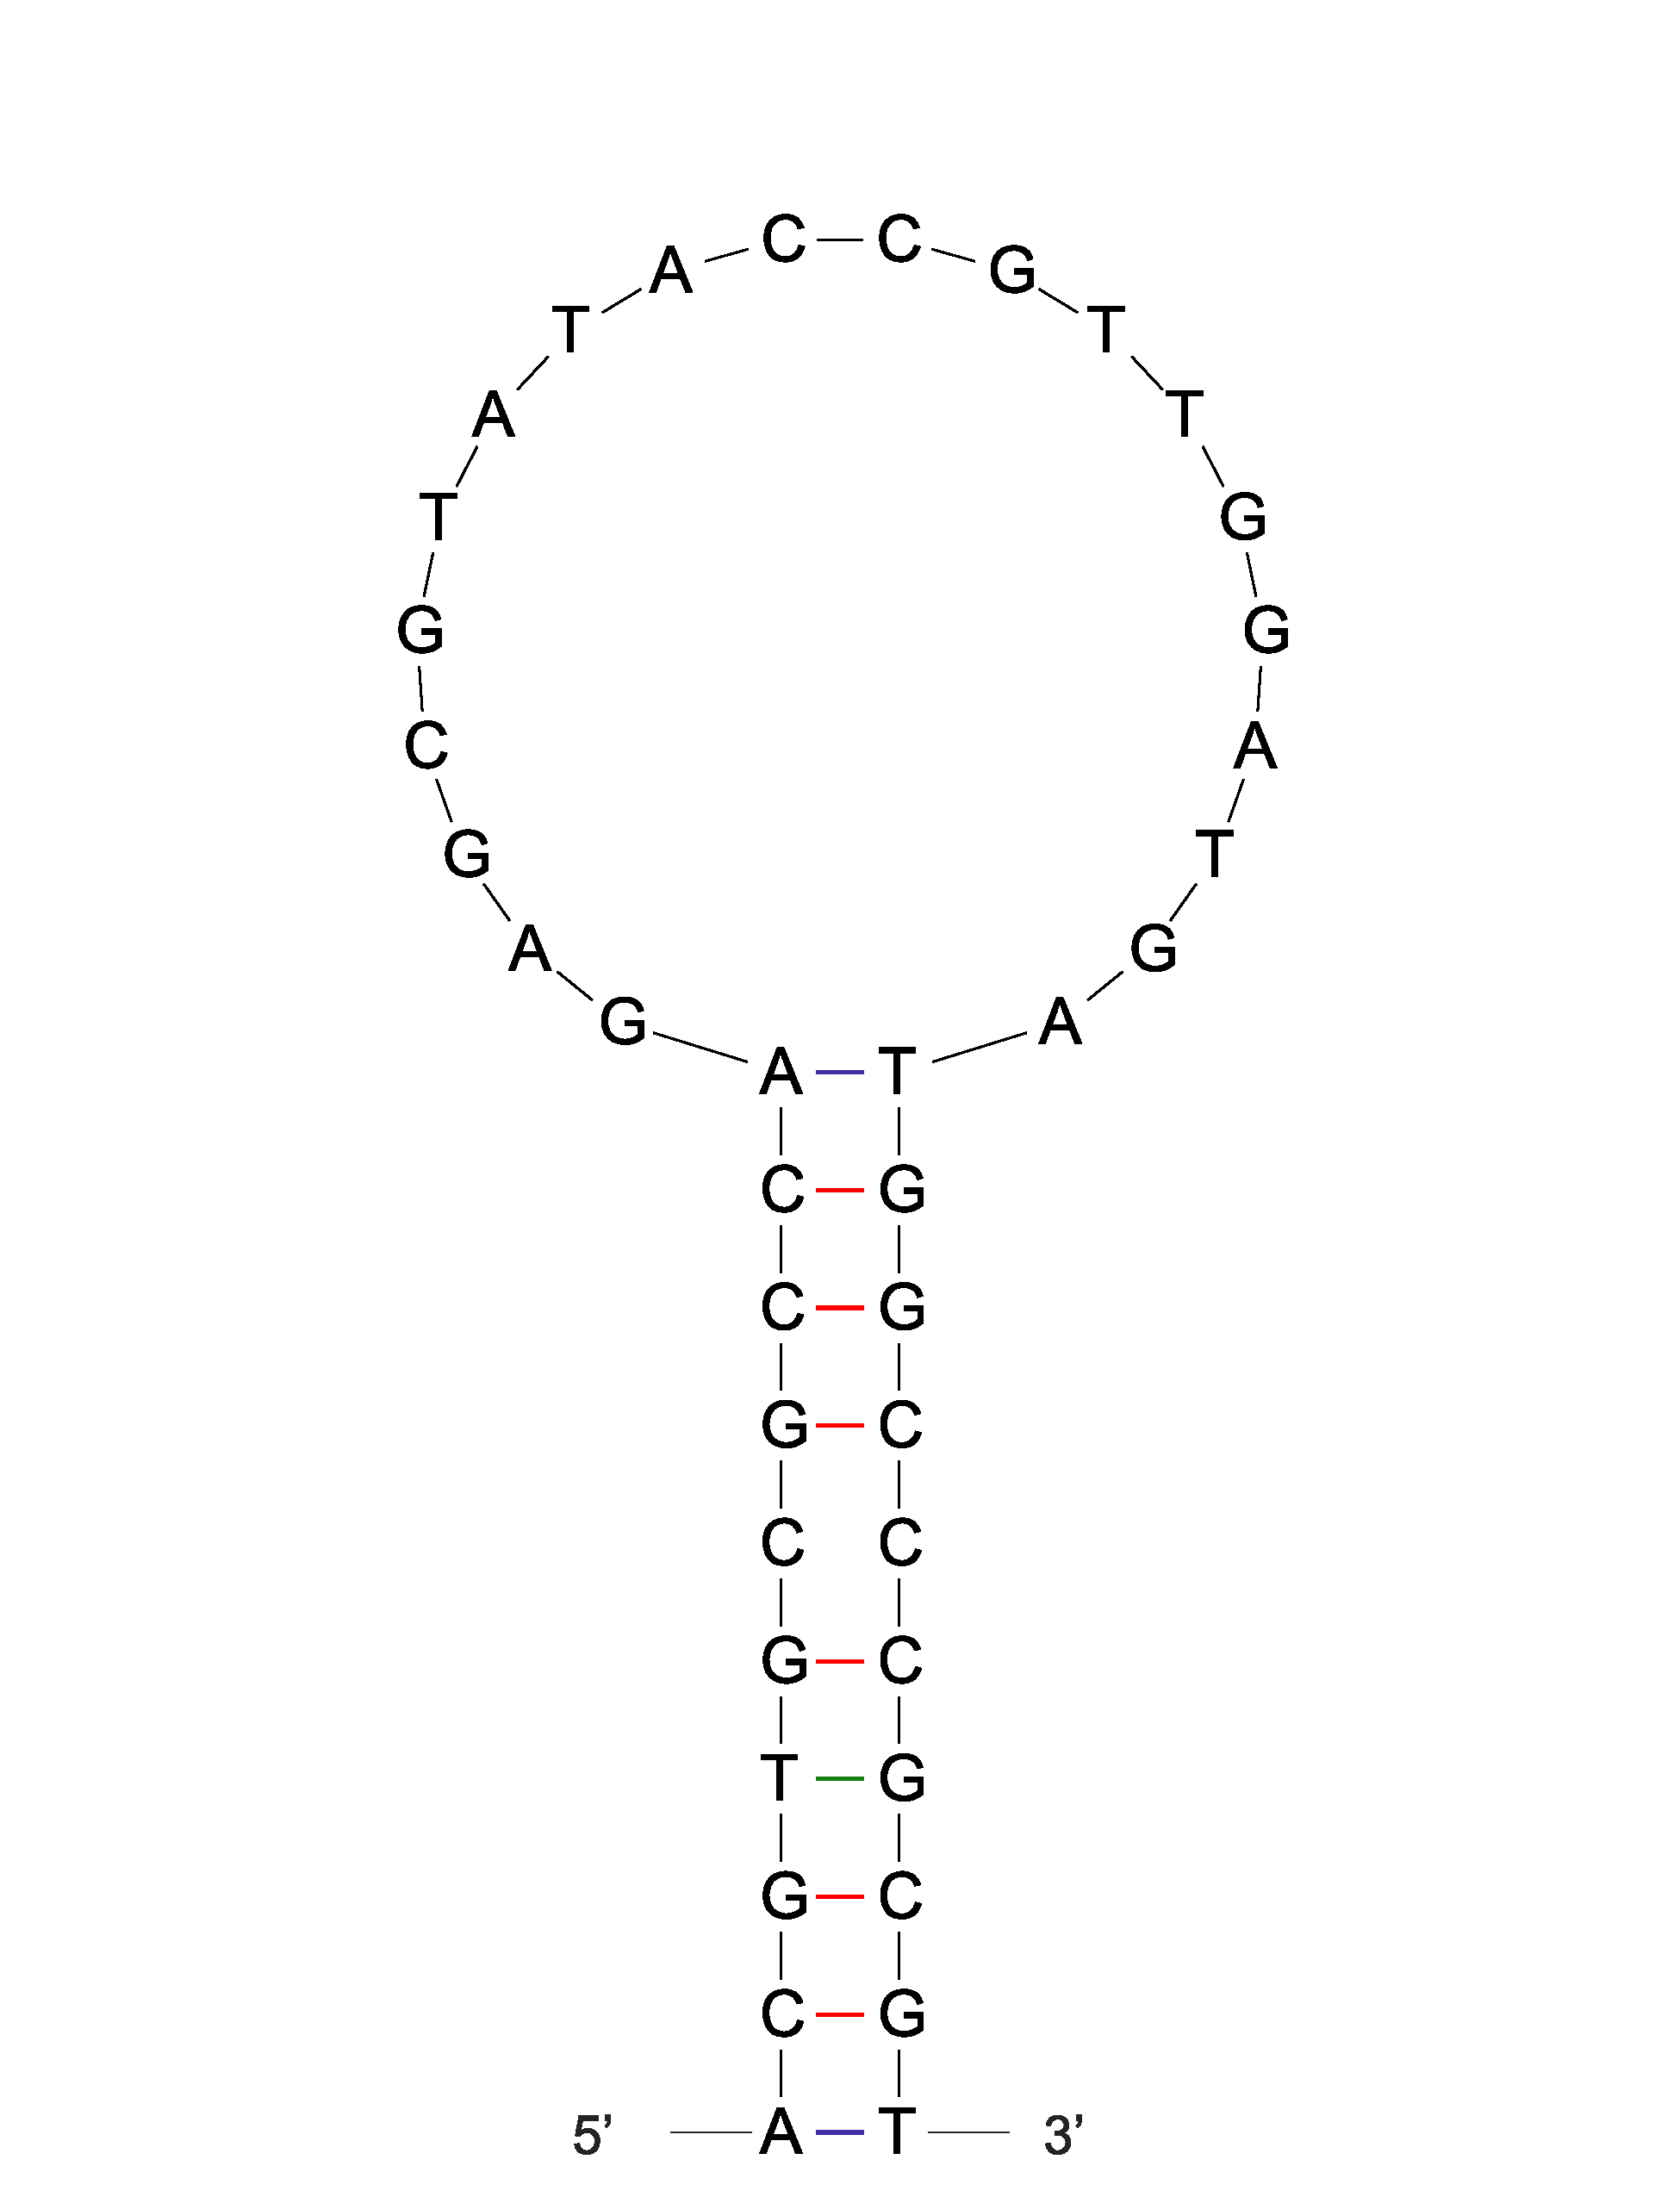
\includegraphics[width=0.3\textwidth]{figures/chapter1/sensors/Fig1_Aptamer.pdf}
        \label{fig:apta}
    }
    \caption{This figure depicts five different types of recognition elements commonly employed in sensors and biosensors:
    (a) Nanozymes are metal nanoparticles with enzyme-like properties: the most common nanozyme activities are here shown, \ie{} oxidase, catalase, peroxidase, and superoxide dismutase.
    (b) Molecularly imprinted polymers (MIPs) are synthetic recognition elements synthesized through the polymerization of functional monomers around a template molecule; the template is then removed leaving highly specific binding sites for the target analyte.
    (c) Antibodies are molecules of the immune system, widely used for their high specificity in binding to target antigens. They are proteins assembled in a Y shape composed of two light and two heavy chains connected by disulfide bonds. The target analyte binds the antibody in the paratope portion, \ie{} at the antigen-binding sites.  
    (d) Enzymes are proteins able to selectively catalyze reactions upon their targets. Here is depicted the three-dimensional crystal structure of \textit{E.coli} catalase (PDB ID: 1IPH). Retrieved from the Protein Data Bank \citep{bravoCrystal1995,bravoRCSB}.
    (e) Aptamers are short, single-stranded oligonucleotides that can fold into specific structures, enabling them to bind to target molecules with high affinity, offering a versatile alternative to antibodies in sensor design.}
    \label{fig:recognitionElements}
\end{figure}

\paragraph{Advantages and limitations of sensors and biosensors}
Sensors and biosensors are superior than traditional detection methods for foodborne hazards, especially in terms of higher sensitivity, miniaturization, cost-effectiveness and user-friendly interfaces \citep{perfezouCancer2012,cardenosa-rubioRecent2019,yangDynamic2022}. These characteristics make them ideal for field applications, thus reducing the need to send samples to laboratories and greatly decreasing the time needed for the analyses \citep{byrneAntibodyBased2009,sonPortable2017,zhangApplying2017}. Sensors are also usually fabricated in such a way that they require little to no sample preparation, \eg{} through the use of microfluidics systems, thus representing a more convenient approach to foodborne hazard detection \citep{hendricksonSensitive2021,liRapid2021}.

However, these technologies are not without disadvantages. Sensors often require complex calibration processes, which can be time-consuming and require skilled expertise \citep{yangCNNLSTM2020}. Moreover, the accuracy of sensors can be reduced in complex food matrices, due to interfering substances that may spoil the analyte signal \citep{gillibertSurface2017,hanRatiometric2021}.
For these reasons, continued research and innovation are essential to optimize sensor performance and improve accessibility.
